
 The function $f(x_1,x_2) = x_1^2 +x_2^2 -2x_1 x_2$ is a continuous function, because it is the sum of continuous functions.

\begin{center}
  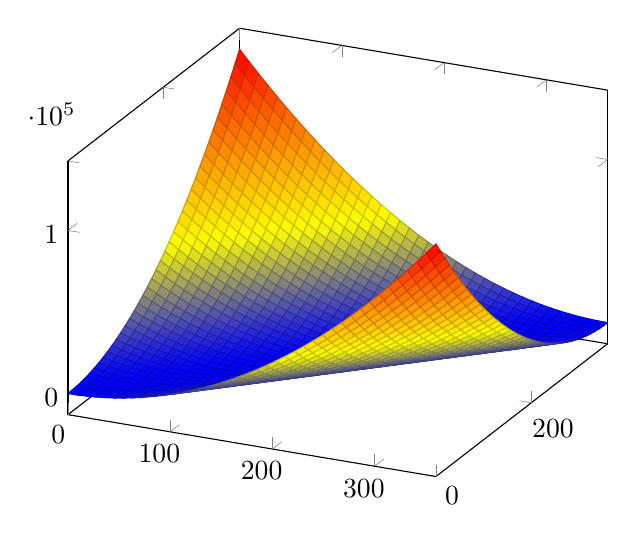
\begin{tikzpicture}
      \begin{axis}
     \addplot3[surf,domain=0:360,samples=40]
      {x^2+y^2-2*x*y};
      \end{axis}
   \end{tikzpicture}
\end{center}

The set $A=\big\{(x_1,x_2) \in \mathbb{R}^2|(x_1-1)^2+(x_2-2)^2 \leq 1 \big\}$ is a compact set:

\begin{center}
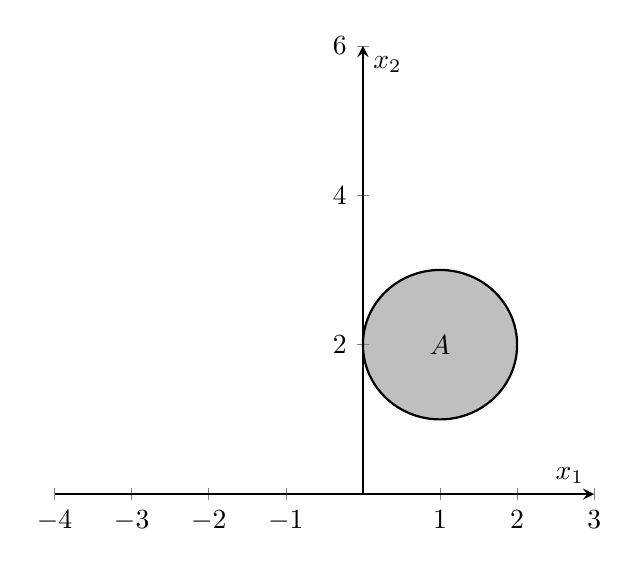
\begin{tikzpicture}
\begin{axis}[ xlabel={$x_1$}, ylabel={$x_2$}
,axis on top=true
,axis lines=middle
,samples=41, thick
,domain=-4:4, xmin=-4, xmax=3,
    ymin=0, ymax=6,
]
   \draw[fill=gray!50] (1,2) circle [radius=1];
\node at (axis cs:1,2) {$A$};   \end{axis}
\end{tikzpicture}
\end{center}

Weierstrass's theorem guarantees that the given function has both a
maximum and a minimum when optimized on the feasible set $A$.

